\chapter{Úvod}
Přísloví praví \uv{Kolik řečí znáš, tolikrát jsi člověkem}. Schopnost dorozumět se s ostatními lidmi na planetě je nesmírně důležitá. Následkem nedorozumění a nepochopení, způsobených mimo jiné i jazykovou bariérou, je mnoho různých konfliktů a problémů. I proto od počátků vzniku výpočetní techniky vědci zkoumají jak vytvořit použitelný překladový systém. Ještě před tím vznikaly a stále vznikají jednoduché tištěné slovníky obsahující překlady jednotlivých slov.

Ideálem je překlad tak jak ho známe ze science fiction materiálů. Dvě osoby, mluvící kompletně jiným jazykem si navzájem rozumí v reálném čase. S rozvojem výpočetní techniky, strojového učení a nástupem umělé inteligence používající hlubokých neuronových sítí se k tomuto ideálu blížíme mílovými kroky. V použitém příkladu je kromě překladu jako takového zahrnuto rozpoznávání řeči a generování. Určování slov jazyku z mluvené řeči, stejně jako generování syntaktické řeči také je možné provádět pomocí neuronových sítí.

Obsahem této práce je však pouze překlad textů z jednoho jazyka do jazyka jiného. A to pomocí nejnovějších metod, objevených a široce nasazovaných v posledních letech, používajících rekurentní neuronové sítě.

V kapitole \ref{chapter:draft} je naformálně nastíněn návrh a cíl této práce. V následující kapitole jsou pak rozebrány důležité pojmy a teorie ze kterých je tato práce vystavěna.

\chapter{Neformální návrh systému} \label{chapter:draft}
Cílem této práce práce je vytvořit systém pro strojový překlad textu pomocí umělých neuronových sítí. Pro snadnou představu, je to podobné jako to co dělá Google Translator\footnote{translate.google.cz} -- blíže popsáno v článku \cite{googleBridgingGap}. Vezme se věta v původním jazyce a vytvoří se z ní co nejvěrnější překlad v jazyce cílovém a to za pomocí natrénované neuronové sítě. V této kapitole je vysvětleno jak by takový systém mohl vypadat a co za komponenty potřebuje k tomu aby fungoval.

\begin{description}
  \item[Dataset:] Aby bylo možné něco překládat, je nejprve zapotřebí mít nějaký dataset. Dataset obsahuje texty ve dvou jazycích mezi kterými se má překládat. Tyto texty musí být zarovnané, tak aby si jednotlivé věty v těchto jazycích navzájem odpovídaly. Obecně platí, že čím větší množství použitých dat a čím větší model, tím lepší bude výsledek.Použít nebo ne?\cite{googleLimits}
      \todo{v kapitole o implementaci pak dát znázorňující obrázek}

  \item[Tokenizer:] Dataset a jeho jednotlivé věty před začátkem trénování sitě je nejprve potřeba připravit. Tokenizer rozdělí věty na jednotlivé tokeny \todo{obrázek ukázky tokenizace}. To usnadňuje práci s datasety a také například snižuje velikost slovníků.

  \item[Slovník:] Slovník se vytvoří jako seznam n nejčastějších slov v datasetu ve vstupním a cílovém jazyce. Čím je slovník menší, tím se zmenší výpočetní požadavky, ale na druhou stranu je potřeba vyřešit při trénování a překladu problém se slovy mimo slovník (OOV -- out of vocabulary). \todo{kde budou popsány unk symbol a tak..v implementaci?}

  \item[Word Embeddings:] Obecně je možné vytvářet jazykové modely, které generují text po písmenech, částech slov nebo po slovech \cite{mikolovSubwords}. V této práci se bude pracovat s celými slovy (tokeny). Word Embeddings je další forma předzpracování. Každý token ze vstupního slovníku se převede do vektoru reálných čísel, ve kterém jsou zakódovány některé syntaktické a sémantické vlastnosti daného tokenu, což umožní neuronové síti se učit lépe, než kdyby se použilo například jenom číslo označující pozici tokenu ve slovníku. \todo{nějaká sekce o slovnících?} Více v sekci \ref{subsection:neuralembeddings}.

  \item[Model:] Pro překlad je nejvhodnějším modelem sequence to sequence (dále seq2seq \cite{seq2seq}) s použitím encoder-decoder architektury. Na rozdíl od starších statistických metod překladu, kde se překládalo po frázích, moderní překlad pomocí neuronových sítí probíhá po celých sekvencích (větách). Nejprve enkodér vezme word embedding na vstupu a pomocí rekurentní neuronové sítě (\ref{section:rnn}) převede větu na vstupu do velkého vektoru reprezentující její význam (tzv. myšlenkový vektor -- intuice je taková, že když člověk překládá větu, také nejprve pochopí její význam a poté ji až začne překládat). Dekodér -- taky rekurentní neuronová síť -- následně z tohoto vektoru slovo po slovu vygeneruje výslednou přeloženou větu. Dekodér tedy funguje jako jazykový model (sekce \ref{section:langmodel}), který je na inicializovaný na jednu konkrétní větu.
\end{description}


\begin{figure}[h]
    \begin{center}
            \tmpframe{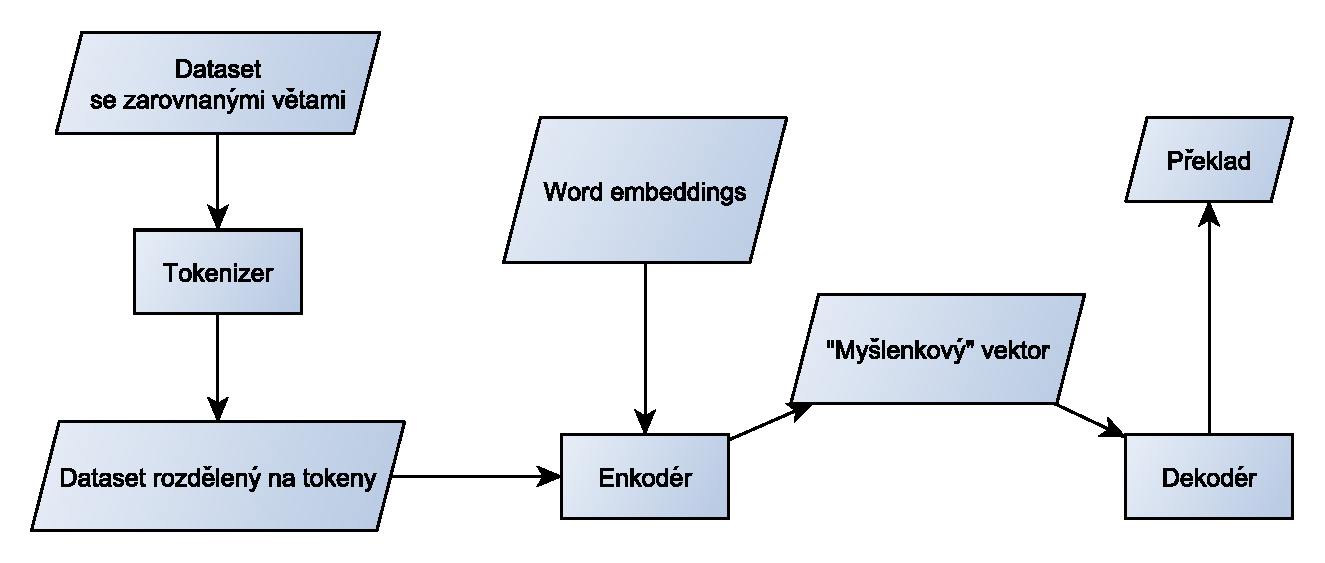
\includegraphics[width=1.0\linewidth]{img/draft.png}}
    \end{center}
	\caption{schéma návrhu systému pro překlad, \todo{obrazek a kompletni popis}}
	\label{img:draft}
\end{figure}


\chapter{Související teorie a pojmy}
Účelem této kapitoly je blíže vysvětlit a rozebrat jednotlivé pojmy a komponenty potřebné pro vytvoření překladového systému.



\section{Jazykové modely}\label{section:langmodel}
Zatímco u programovacích jazyků existuje jejich formální definice, přesně popisující jejich syntaxy a význam, u přirozených jazyků to tak není. Přirozený jazyk vznikl náhodným způsobem v průběhu staletí a tisíciletí narozdíl od formálně definovaných jazyků, které byly přímo navrženy. Přestože běžný jazyk se řídí nějakými pravidly, existuje značné množství výjimek a odchylek. I napříč tomu si však lidé navzájem rozumí. Problém však je tyto pravidla převést do formálních pravidel, tak aby jim rozuměl počítač. Řešením pro tento problém mohou být jazykové modely, které nevznikají nadefinováním formálních pravidel, nýbrž nacvičením se z příkladů. Sekce vychází z práce \cite{nmtThesis} a článku \cite{nmtTutorial}.
\\\\
Jazykový model udává pro každou větu $w$ jaká je její pravděpodobnost. Respektive pro sekvenci slov $w = w_1, w_2..., w_m$ získá pravděpodobnost podle rovnice \ref{figure:probdistr}.

\begin{align}\label{figure:probdistr}
  p(w) = \prod_{i=1}^{m} p(w_i|w_{<i})
\end{align}

Pro každé slovo $w_i$ ze sekvence $w$ určí jaká je jeho podmíněná pravděpodobnost v případě, že se před ním nachází slova $w_{<i}$.

\subsection{N-gram modely}\label{subsection:ngram}
Ve výsledku je pro překladový systém potřeba získat model, který pro zdrojovou větu $E$ vrátí přeloženou větu $F$, tak že $P(F|E)$. N-gram model je však jazykový model, který udává jen pro pravděpodobnost věty P(F) (pro nějaký daný kontext nad kterým se model nacvičil). 

Takovýto model umožní zhodnotit přirozenost věty a generovat text podobný tomu, na kterém byl model nacvičen \cite{nmtTutorial}.

\begin{description}
  \item[Zhodnocení přirozenosti:] Pomocí jazykového modelu je možné pro větu $w$ zhodnotit, jak moc je přirozená nebo-li jak moc je pravděpodobné, že by takováto věta mohla existovat v textu na kterém byl model nacvičen.
  \item[Generování textu:] Protože model umožňuje pro každé slovo $w_i$ získat pravděpodobnost následujícího slova $w_{i+1}$, je takto možné generovat náhodný, přirozeně (vůči zdrojovému textu) vypadající text. Přesně tato vlastnost je potřeba pro generování překladů.
\end{description}

$N$-gram modely umožňují určit pravděpodobnost následujícího slova ve větě v případě, že se před ním nacházelo $n$ nějakých slov (rovnice \ref{figure:ngram}).

\begin{align}\label{figure:ngram}
    P(x_{i}\mid x_{{i-(n-1)}},\dots ,x_{{i-1}})
\end{align}

Se zvětšujícím se $n$ se výrazně zvětšuje náročnost výpočtu. Tímto způsobem tak není snadné zachytit závislosti mezi slovy vzdálenými od sebe více než pár míst.

\subsection{Log-linearání modely} \label{subsection:loglinear}
Stejně jako v případě $n$-gram modelů (sekce \ref{subsection:ngram}), tyto modely počítají pravděpodobnost následujícího slova $w_i$ při kontextu $w_{<i}$. $n$-gram model počítá pouze s výskytem (identitou) slova. Log-lineární modely pracují s \textbf{rysy} (z anglického features). Rys je něco užitečného ohledně daného slova, co se dá použít pro zapamatování a pro předpověď slova dalšího. Jak už bylo řečeno, u n-gram modelů to je identita minulého slova. Formálněji je rys funkce $\phi(e^{t-1}_{t-n+1})$, která dostane na vstupu aktuální kontext a jako výsledek vrátí reálnou hodnotu -- vektor rysů $x \in \mathbb{R}^N$ popisující kontext při použití $N$ různých rysů.

Stejně jako u $n$-gram modelů, nastává problém když je potřeba zaznamenat vzdálenější závislosti. Například u věty \uv{farmář jí steak} je potřeba zaznamenat pro předpovězení slova \uv{steak} jak jeho předcházející slovo $w_{t_1}=j\acute{\imath}$, tak $w_{t_2}=farm\acute{a}\check{r}$. V případě, že by se použil pouze rys $w_{t_1}$, mohl by model předpovídat i věty, které nedávají smysl. Jako je například \uv{kráva jí steak}. Při použití většího množství rysů vznikají mnohem větší nároky na paměť a výkon a taky na velikost trénovacího datasetu. Řešením těchto problémů může být použití neuronových sítí (sekce \ref{subsection:neuralembeddings}).


\subsection{Neuronové sítě a word embeddings}\label{subsection:neuralembeddings}
Stejně jako předchozí modely i NLM (neural language model) je trénován tak aby předpovídal rozložení pravděpodobností přes slova v cílovém slovníku na základě aktuálního kontextu (rovnice \ref{figure:probdistr}).

Předchozí modely při použití většího datasetu a tím pádem většího slovníku čelí \uv{prokletí} dimenzionality. Jednotlivá slova jsou běžně reprezentována jako \textbf{one-hot vector} \todo{obrázek s ukázkou}. Pro reprezentaci jednoho slova je tak použit rozsáhlý vektor $x_i \in \mathbb{R}^{V}$, kde $V$ je použitý slovník daného jazyka. Většina hodnot, až na hodnotu označující dané slovo, je nulová (řídký vektor nebo-li sparse vector).

NLM se s tímto problémem vypořádává za pomocí takzvaných \textbf{word embeddings}. Word embeddings, jsou na rozdíl od one-hot vektoru vektory reálných čísel (husté nebo-li dense vektory). Ke každému slovu ze slovníku se přiřadí takovýto vektor. Výhodou je, že může nést, narozdíl od pouhé pozice slova ve slovníku, další různé užitečné významy. Třeba pro slovo \uv{kráva}, by ve vektoru mohly být zakódovné významy jako podstatné jméno, velký savec atd. Díky tomu může model lépe generalizovat, a slova, která jsou sobě blízká v tomto prostoru, může model brát například jako synonyma.
Nejznámější ukázkou vlastností word embeddings je ukázka \ref{figure:kingQueen} z článku \cite{kingQueen}.

\begin{align}\label{figure:kingQueen}
  v(kr\acute{a}l) - v(mu\check{z}) + v(\check{z}ena) \approx v(kr\acute{a}lovna)
\end{align}

$\approx$ udává nejbližšího souseda v prostoru. Je vidět, že vektory v sobě nesou určitý sémantický význam. Odečtením hodnoty vektoru slova \uv{muž} se získá jakási podstata slova \uv{král} nebo \uv{kralovat}. Přičtením hodnoty slova \uv{žená} k této dočasné hodnotě se pak získá ženská varianta krále -- královna.

\todo{taky dobrej popis nlm a embeddings (distributed representation) \url{http://www.scholarpedia.org/article/Neural_net_language_models}}

\todo{popis toho že řeší problémy co má n-gram (jen pár dozadu, nevím jak přesně?) a log-linear (díky nečemu (embeddings?) to vyloučí špatný kombinace jako kráva žere krávu nebo co (viz tutorial)}


Zmíním co existuje za druhy, lehce jejich rozdíly a vznik (co jsou zač) a pak se víc rozepíšu o fasttextu, protože to je ten co jsem použil (rovnice a kdesi cosi)


bengio neural net language models\cite{Bengio:2008}


Existuje několik moderních variant výpočtů word embeddings:
\begin{itemize}
  \item word2vec \cite{word2vec}
  \item glove  \cite{glove}
  \item fasttext \cite{fasttext}
\end{itemize}

využití transfer learning - použijou se předučený embeddings od jinud pro zlepšení výkonu modelu na překlad

\subsection{Zpracování neznámých slov}
Existuje-li dataset $\varepsilon_{train}$ obsahující texty na kterých se model bude učit a dataset $\varepsilon_{test}$, který bude sloužit k ověření výkonosti a generalizace modelu, je více než pravděpodobně, že v testovacím setu se budou nacházet slova, která se v trénovacím nenacházela. Také může být vhodné omezit celkový počet slov se kterými se bude model trénovat, pro zlepšení výkonu. Práce \cite{nmtTutorial} uvádí tři běžné způsoby jak se vypořádat s takovými \textbf{neznámými slovy}.

\begin{description}
  \item[Předpokládat že slovník je konečně velký:] V některých případech se dá počítat s tím, že slovník je omezený.Tím pádem se neznámá slova nebo znaky nemohou vyskytovat. Například, když by se počítal model učený na znacích ASCII, tak při dostatečně velkém vstupním datasetu by bylo rozumné předpokládat, že se v něm vyskytli a model se tedy mohl naučit všechny znaky.
  \item[Interpolate with an unknown words distribution:] \todo{TODO}
  \item[Přídáním speciálního slova <unk>:]\label{description:unk}V případě, že se v trénovacím setu $\varepsilon_{train}$ některá slova vyskytují málo nebo jenom jednou, mohou se nahradit speciálním slovem \emph{<unk>}. S tímto slovem se pak pracuje stejně jako s ostatními. Díky tomu se zredukuje počet slov ve slovníku a tedy náročnost výpočtu. Má však taky přiřazenou svoji pravděpodobnost a může se tak vyskytnout v předpovědi modelu při generování textu. \todo{odkázat se sem ze sekce kde bude napsaný že tohle je varianta co používám}
\end{description}

\section{Rekurentní neuronové sítě}\label{section:rnn}
V této kapitole je popsán základní koncept rekurentních neuronových sítí (RNN\footnote{z anglického recurrent neural network}), jejich srovnání s běžnými neuronovými sítěmi a dále pak popis upravených variant rekurentních sítí -- LSTM (sekce \ref{section:LSTM}) a GRU (sekce \ref{section:GRU}). Sekce vychází z práce \cite{nmtThesis}, práce \cite{nmtTutorial} a článku \cite{understandingLSTM}.


RNN (Elman \cite{rnn}) jsou známé již přes dvě desítky let. Úspěšně jsou však používány až v posledních letech. A to hlavně díky vyššímu výpočetnímu výkonu a většímu objemu trénovacích dat, který je v současné době dostupný a také zpracovatelný. Tento druh neuronových sítí je obzvlášť vhodný například pro rozpoznávání psaného písma, rozpoznávání řeči, v kombinaci s konvolučními neuronovými sítěmi pro generování popisků obrázků a co je nejvíce zajímavé pro tuto práci, pro tvorbu jazykových modelů, generátorů textu a tím pádem i pro překlad.

Jejich hlavních výhodou oproti jednoduchým dopředným neuronovým sítím je jejich schopnost držet si vnitřní stav napříč časem. Dopředná neuronová síť pracuje vždy s aktuální hodnotou $x$ na vstupu, pro kterou pomocí vah $W$ získá výstup $y$ (rovnice \ref{figure:basic-nn}). 

\begin{align}\label{figure:basic-nn}
  y = f (x, W)
\end{align}

Pokud pak takováto síť pracuje s nějakou sekvencí měnící se v čase, například se slovy v rámci jedné věty, pro každé slovo na vstupu $x_t$, kde $t$ znázorňuje čas (pozici) slova ve větě, použije stejné váhy pro získání výstupu $y_t$ a nezjistí ani nezachová žádnou úvahu o vzájemném vztahu těchto slov.

RNN tento problém řeší zavedením vnitřního stavu $h_t$ a smyčky (obrázek \ref{img:rnn-rolled}). Vstupem dalšího stavu je kromě nového vstupu vždycky také výstup ze stavu minulého. Pro každé $x_t$ ze sekvence se tedy nyní může získat výstup $y_t$ pomocí vnitřního stavu $h_t$ z předchozího kroku $t$ (rovnice \ref{figure:rnn}). Přičemž počáteční stav  $h_0$ je obvykle nastaven na nulu.

\begin{align}\label{figure:rnn}
  h_t = \begin{cases}
          f(W_{xh}x_t + W_{hh}h_{t-1} + b_h) & \mbox{pokud t $\geq$ 1}, \\
          0 & \mbox{jinak}.
        \end{cases}
\end{align}


$W_{xh}$ znázorňuje váhy pro aktuální vstup, $W_{hh}$ jsou váhy pro vnitřní stav z minulého kroku a $b_h$ je bias. Funkce $f$ z rovnice \ref{figure:rnn} je nelineární funkcí a nejčastěji se používá jedna z funkcí \emph{sigmoid}, \emph{tanh} nebo \emph{relu} \ref{img:functions}. \todo{lepe popsat jednotlivé funkce a jejich výhody/nevýhody}

Rovnice pro RNN jazykový model jsou následující:

\begin{align}
  m_{t}&=M_{e_{t-1}}\label{figure:lastContext} \\
  h_{t}&=RNN(m_t, h_{t-1}) \label{figure:rnnSimple} \\
  s_{t}&=W_{hs}h_t + b_s \label{figure:rnnSt} \\
  p_{t}&=softmax(s_t) \label{figure:rnnSoftmax}
\end{align}


Kde \ref{figure:lastContext} je aktuální kontext, \ref{figure:rnnSimple} je zjednodušený přepis rovnice RNN \ref{figure:rnn} a rovnice \ref{figure:rnnSoftmax} je funkce softmax \ref{figure:softmax}, která vezme všechny hodnoty skóre pro jednotlivá slova a transformuje je do pravděpodobnostního rozložení $p_t$. Díky tomu pak lze již snadno určit, které slovo bude vygenerováno s největší pravděpodobností.

\begin{figure}[h]
    \begin{center}
            \tmpframe{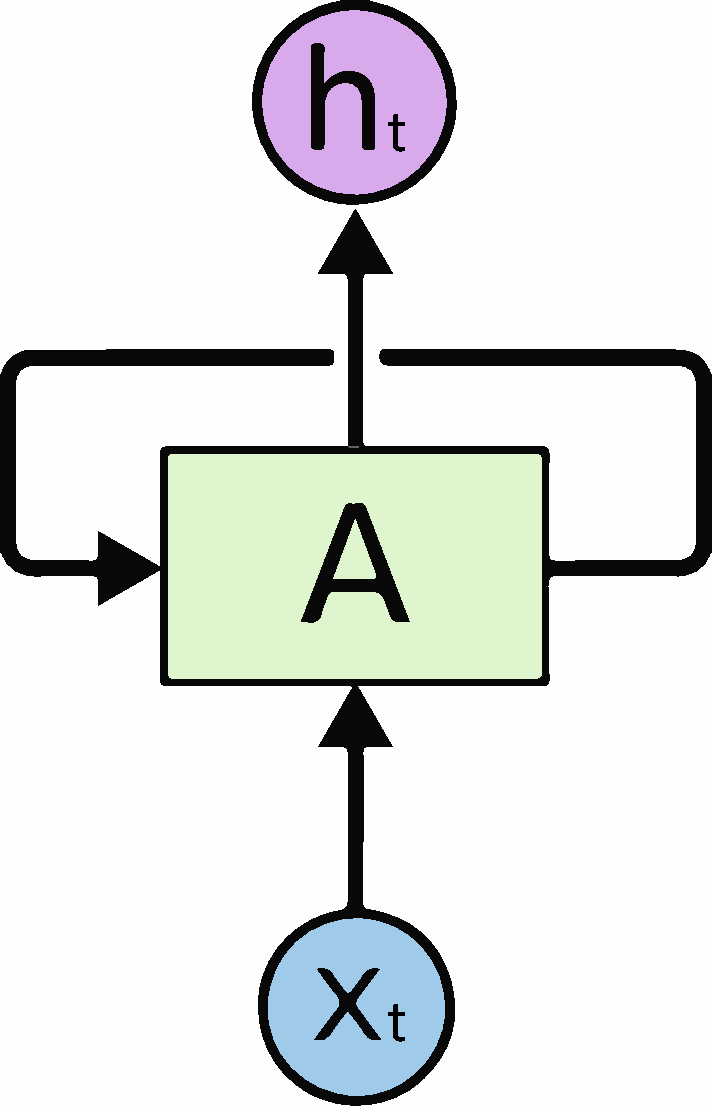
\includegraphics[width=0.3\linewidth]{img/RNN-rolled.png}}
    \end{center}
	\caption{Recurrent Neural Networks have loops. \todo{vlastni obrázek nebo citace \url{http://colah.github.io/posts/2015-08-Understanding-LSTMs/} }}
	\label{img:rnn-rolled}
\end{figure}

\begin{figure}[h]
    \begin{center}
            \tmpframe{\includegraphics[width=0.3\linewidth]{img/placeholder.pdf}}
            \tmpframe{\includegraphics[width=0.3\linewidth]{img/placeholder.pdf}}
            \tmpframe{\includegraphics[width=0.3\linewidth]{img/placeholder.pdf}}
    \end{center}
	\caption{\todo{vedle sebe obrazky funkci relu, tanh, sigmoid, idealne tri ruzny captions}}
	\label{img:functions}
\end{figure}


\begin{align}\label{figure:softmax}
  p_t(y)={\frac {e^{p_{t}(y)}}{\sum _{k=1}^{K}e^{p_{t_{k}}}}}
\end{align}


\begin{figure}[h]
    \begin{center}
            \tmpframe{\includegraphics[width=1.0\linewidth]{img/RNN-unrolled.png}}
    \end{center}
	\caption{A recurrent neural network and the unfolding in time of the computation involved in its forward computation. \todo{vlastni obrázek nebo citace \url{http://colah.github.io/posts/2015-08-Understanding-LSTMs/} }}
	\label{img:rnn}
\end{figure}

Cílem jazykového modelu je předpovídat následující slovo ve větě. Aby model věděl kdy má začít a ukončit predikci, používají se speciální \textbf{počáteční a koncový symbol} (<s>, </s>). Vstupní věta (sekvence) $x$ by například mohla být $x$ = \{<s>, Venku, sedí, kočka\}. Věta $y$ generovaná modelem, by pak mohla být například tatáž věta, ale posunutá o jeden časový úsek dopředu -- $y$ = \{Venku, sedí, kočka, </s>\}. V ilustraci \todo{...} je názorná ukázka.

\begin{figure}
    \begin{center}
            \tmpframe{\includegraphics[width=0.5\linewidth]{img/placeholder.pdf}}
    \end{center}
	\caption{\todo{Obrázek jako je v nmt thesis strana 19, figure 2.3}}
	\label{img:TODO}
\end{figure}



Protože vektor $m$ z rovnice \ref{lastContext} je konkatenací všech předchozích slov (a tedy je to aktuální kontext), model se může naučit kombinací různých vlastností napříč několika různými slovy z kontextu. V sekci \ref{subsection:loglinear} byl jako problém uveden příklad \uv{Farmář jí maso} a \uv{Kráva jí maso}, kde druhá věta nedává smysl. Při použití RNN by se pro kontext $M_f$ obsahující {farmář, jí} mohla naučit jedna z jednotek skryté vrstvy $h$ rozpoznat vlastnost "věci které farmář jí" a správně se aktivovat a pak nabízet slova jako \uv{maso} nebo \uv{brambory}. Zatímco pro kontext $M_k$ {kráva, jí} by jiná se naučila zase jiná jednotka. RNN je tedy schopná zachytit vzdálené závislosti jako je \todo{obrázek s textem znázorňujícím long-distance dependency, viz tutorial Sekce 6, figure 14 a i ten text pod tim kde je to dobre rozepsany}. Základní verze RNN je však schopná zachytit závislosti jen do určité vzdálenosti viz \ref{subsection:gradient}.


\todo{doplnit rovnice (patrne z tutorialu) a vysvětlení jak se to aplikuje dál, stejně tak obrázky s unrolled rnn a popisem toho jak zachovává nějakou informaci (třeba že podstatné jméno je mužské) skrze jednotlivé kroky (i když ne úplně přes vzdálené a tím se dostanu k long term dependencies)}

\todo{predchazeni vanish/exploding - lstm a gru, ktery s tim nejak pocitaji. Regularization - vysvětlit co to je}
\todo{deep, bi-directional}


\subsection{Mizející a explodující gradient} \label{subsection:gradient}
RNN jsou oproti základním neuronovým sítím schopné zachytit různé závislosti mezi slovy na delší vzdálenosti. I tato schopnost je však velmi limitovaná. Hlavními zdroji problémů jsou \textbf{mizející a explodující gradient} (článek \cite{gradientProblems}). 

\todo{patrne v nejake predchozi casti zhruba popsat LOSS, BACKPROPAGATION aby se tady na to pak dalo navazat}

Při průběhu učení RNN průběžně vznikají predikce a počítá se \emph{loss} \todo{kde je popsaná} funkce. Následně je potřeba zpětně zpropagovat tuto hodnotu přes všechny (časové) kroky sítě (Back propagation over time -- BPTT). Pokud však není gradient rovný 1, tak se v každém zpětném kroku buďto zmenší a tím pádem se blíží k nule, nebo se naopak zvětší a blíží s k nekonečnu. Ve výsledku je tak gradient buďto příliš malý a nemá tak tak žádný efekt na úpravu vah nebo jimi pohne příliš a tak zaviní špatné učení se sítě.

\begin{figure}
    \begin{center}
            \tmpframe{\includegraphics[width=0.5\linewidth]{img/placeholder.pdf}}
    \end{center}
	\caption{\todo{ukázka problémů s gradientem, něco jako figure 16 v 6.3 tutorialu}}
	\label{img:TODO}
\end{figure}

Jako možné řešení těchto problémů vznikla varianta rekurentní sítě LSTM \ref{section:LSTM}.




\subsection{LSTM}\label{section:LSTM}
Long short term memory (článek \cite{LSTM}, dále LSTM) nebo-li dlouhá krátkodobá paměť, je varianta RNN řešící problém mizejícího gradientu a vzdálených závislostí \todo{lepší překlad pro long term dependencies?}.

\begin{align}
    f_{t}&=\sigma _{g}(W_{xf}x_{t}+W_{hf}h_{t-1}+b_{f})\\
    i_{t}&=\sigma _{g}(W_{xi}x_{t}+W_{hi}h_{t-1}+b_{i})\\
    o_{t}&=\sigma _{g}(W_{xo}x_{t}+W_{ho}h_{t-1}+b_{o})\\
    c_{t}&=f_{t}\circ c_{t-1}+i_{t}\circ \sigma_{c}(W_{c}x_{t}+U_{c}h_{t-1}+b_{c})\\
    h_{t}&=o_{t}\circ \sigma _{h}(c_{t})
\end{align}

\subsection{GRU}\label{section:GRU}


\subsection{Trénování}
\todo{trénování rnn, back propagation through time, have difficulties (\url{http://proceedings.mlr.press/v28/pascanu13.pdf}) learning long term dependencies}
\todo{loss computing}
\todo{gradient computing}

\subsection{Global optimization methods viz wiki on RNN}




\section{Modely seq2seq}


\subsection{Encoder-decoder architektura}
\begin{figure}
    \begin{center}
            \tmpframe{\includegraphics[width=0.5\linewidth]{img/placeholder.pdf}}
    \end{center}
	\caption{One image. \todo{Napsat pořádný titulek}}
	\label{img:TODO}
\end{figure}




Ne jako samostatná kapitola, ale v rámci nějaké (asi implementace) bych udělal itemize a nebo přinejmenším aspon zběžně popsal proč jsem zvolili Keras.
\emph{Frameworky}
\begin{itemize}
  \item Tensorflow
  \item Theano
  \item CNTK
  \item Keras
\end{itemize}


\chapter{Implementace}
Naprogramoval jsem.
Posbíral jsem data.
Pustil jsem to.
Výsledky jsou takové.
Je to tak a tak rychlé.

\section{Baseline systém v Moses}
\todo{Jak rozlišit návrh a realizaci?}
\blind{3}

\section{Dataset/y}
Jejich struktura, jak je zpracuji a použiji
\blind{2}
\begin{figure}
    \begin{center}
            \tmpframe{\includegraphics[width=0.5\linewidth]{img/placeholder.pdf}}
    \end{center}
	\caption{One image. \todo{ukázka ze souborů různých jazyků z jednoho datasetu}}
	\label{img:TODO}
\end{figure}


\subsection{Bucketing}
A padding. Rozdělení sekvencí na skupiny podle délky, abych nepaddingoval zbytečně a tím neplýtval výkon. \todo{porovnat čas jaký to běží a rozdíl v přenosti překladu vůči bez bucketingu}

\section{Generování encoded vět aby se vešly do paměti}

\section{popis fungování systému a jednotlivých tříd}
\todo{zkusit nějak použit vygenerovanou dokumentaci? nebo aspon do příloh}

\chapter{Experimenty a vyhodnocení}
\section{skóre BLEU}
\blind{1}
\todo{vysazet hezky vzorce}



\chapter{Závěr}
\begin{itemize}
  \item Autor se ohlíží za tím, co udělal: „V práci je. Hlavní úspěchy jsou. Důležitými výsledky jsou. Podařilo se.“
  \item Autor uvede nápady, které nestihl realizovat v podobě možností pokračování: „Ještě by šlo zkusit. Kdybych byl na začátku věděl, co vím teď, dělal bych.“
  \item Autor (ve vlastním zájmu) rekapituluje, jak bylo naplněno zadání práce.
\end{itemize}

\textbf{Plány do budoucna}
\begin{itemize}
    \item použití bidirectional první vrstvy encoderu, pro lepší zachování contextu \cite{googleBridgingGap} na místo použití obrácených vstupů
    \item použití wordpieces \cite{googleBridgingGap} místo celých slov pro lepší handling rare words
    \item přidat attention \cite{attention}
    \item přidat beam search \cite{nmtTutorial}, sehnat původní článek co přinesl beam search
\end{itemize}
